\documentclass{standalone}
\usepackage{tikz}
\usetikzlibrary{patterns, positioning}


\begin{document}
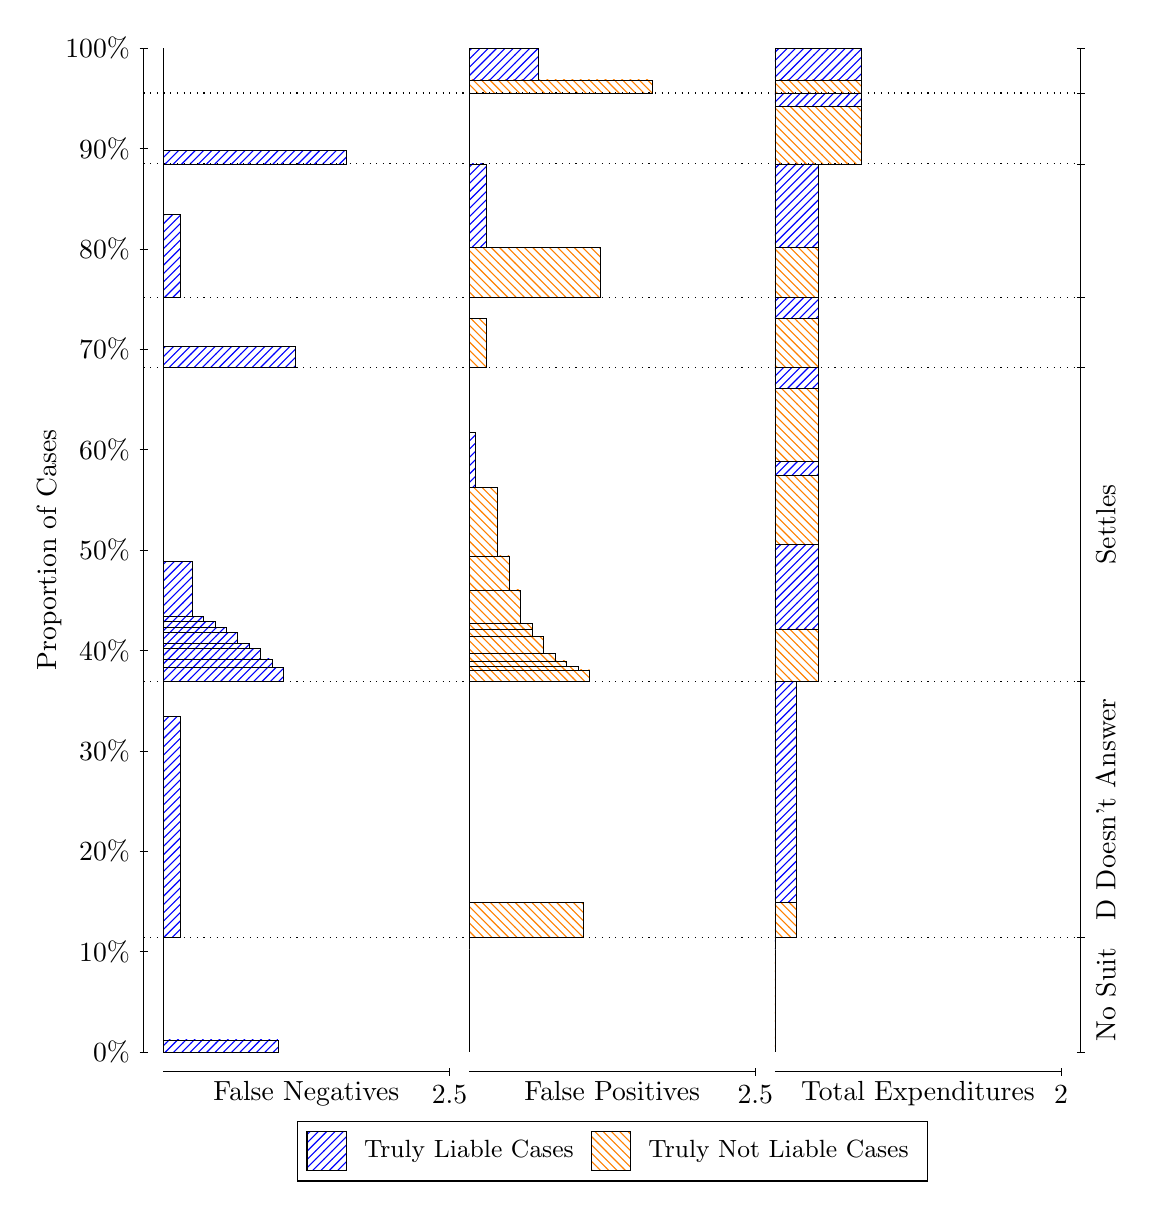
\begin{tikzpicture}
\draw[black, very thin] (1.5,1.75) -- (1.5,14.5);
\node[rotate=90, text=black, anchor=center] at (0.3, 8.125) {Proportion of Cases};
\draw[black, very thin] (1.45,1.75) -- (1.55,1.75);
\node[text=black, anchor=east] at (1.45, 1.75) {0\%};
\draw[black, very thin] (1.45,3.025) -- (1.55,3.025);
\node[text=black, anchor=east] at (1.45, 3.025) {10\%};
\draw[black, very thin] (1.45,4.3) -- (1.55,4.3);
\node[text=black, anchor=east] at (1.45, 4.3) {20\%};
\draw[black, very thin] (1.45,5.575) -- (1.55,5.575);
\node[text=black, anchor=east] at (1.45, 5.575) {30\%};
\draw[black, very thin] (1.45,6.85) -- (1.55,6.85);
\node[text=black, anchor=east] at (1.45, 6.85) {40\%};
\draw[black, very thin] (1.45,8.125) -- (1.55,8.125);
\node[text=black, anchor=east] at (1.45, 8.125) {50\%};
\draw[black, very thin] (1.45,9.4) -- (1.55,9.4);
\node[text=black, anchor=east] at (1.45, 9.4) {60\%};
\draw[black, very thin] (1.45,10.675) -- (1.55,10.675);
\node[text=black, anchor=east] at (1.45, 10.675) {70\%};
\draw[black, very thin] (1.45,11.95) -- (1.55,11.95);
\node[text=black, anchor=east] at (1.45, 11.95) {80\%};
\draw[black, very thin] (1.45,13.225) -- (1.55,13.225);
\node[text=black, anchor=east] at (1.45, 13.225) {90\%};
\draw[black, very thin] (1.45,14.5) -- (1.55,14.5);
\node[text=black, anchor=east] at (1.45, 14.5) {100\%};

\draw[black, very thin] (13.4,1.75) -- (13.4,14.5);
\draw[black, very thin] (13.35,1.75) -- (13.45,1.75);
\node[anchor=west] at (13.35, 1.75) {};
\draw[black, very thin] (13.35,3.2067) -- (13.45,3.2067);
\node[anchor=west] at (13.35, 3.2067) {};
\draw[black, very thin] (13.35,6.452) -- (13.45,6.452);
\node[anchor=west] at (13.35, 6.452) {};
\draw[black, very thin] (13.35,10.447) -- (13.45,10.447);
\node[anchor=west] at (13.35, 10.447) {};
\draw[black, very thin] (13.35,11.329) -- (13.45,11.329);
\node[anchor=west] at (13.35, 11.329) {};
\draw[black, very thin] (13.35,13.03) -- (13.45,13.03);
\node[anchor=west] at (13.35, 13.03) {};
\draw[black, very thin] (13.35,13.929) -- (13.45,13.929);
\node[anchor=west] at (13.35, 13.929) {};
\draw[black, very thin] (13.35,14.5) -- (13.45,14.5);
\node[anchor=west] at (13.35, 14.5) {};

\draw[black, very thin, pattern color=blue, pattern=north east lines] (1.75,1.75) rectangle (3.2033,1.9033);
\draw[black, very thin, pattern color=orange, pattern=north west lines] (1.75,1.9033) rectangle (1.75,3.2067);
\draw[black, very thin, pattern color=blue, pattern=north east lines] (1.75,3.2067) rectangle (1.968,6.0125);
\draw[black, very thin, pattern color=orange, pattern=north west lines] (1.75,6.0125) rectangle (1.75,6.452);
\draw[black, very thin, pattern color=blue, pattern=north east lines] (1.75,6.452) rectangle (3.276,6.634);
\draw[black, very thin, pattern color=blue, pattern=north east lines] (1.75,6.634) rectangle (3.1307,6.7431);
\draw[black, very thin, pattern color=blue, pattern=north east lines] (1.75,6.7431) rectangle (2.9853,6.8774);
\draw[black, very thin, pattern color=blue, pattern=north east lines] (1.75,6.8774) rectangle (2.84,6.9429);
\draw[black, very thin, pattern color=blue, pattern=north east lines] (1.75,6.9429) rectangle (2.6947,7.0754);
\draw[black, very thin, pattern color=blue, pattern=north east lines] (1.75,7.0754) rectangle (2.5493,7.1441);
\draw[black, very thin, pattern color=blue, pattern=north east lines] (1.75,7.1441) rectangle (2.404,7.2226);
\draw[black, very thin, pattern color=blue, pattern=north east lines] (1.75,7.2226) rectangle (2.2587,7.2848);
\draw[black, very thin, pattern color=blue, pattern=north east lines] (1.75,7.2848) rectangle (2.1133,7.9773);
\draw[black, very thin, pattern color=orange, pattern=north west lines] (1.75,7.9773) rectangle (1.75,10.447);
\draw[black, very thin, pattern color=blue, pattern=north east lines] (1.75,10.447) rectangle (3.4213,10.707);
\draw[black, very thin, pattern color=orange, pattern=north west lines] (1.75,10.707) rectangle (1.75,11.329);
\draw[black, very thin, pattern color=blue, pattern=north east lines] (1.75,11.329) rectangle (1.968,12.387);
\draw[black, very thin, pattern color=orange, pattern=north west lines] (1.75,12.387) rectangle (1.75,13.03);
\draw[black, very thin, pattern color=blue, pattern=north east lines] (1.75,13.03) rectangle (4.0753,13.198);
\draw[black, very thin, pattern color=orange, pattern=north west lines] (1.75,13.198) rectangle (1.75,13.929);
\draw[black, very thin, pattern color=orange, pattern=north west lines] (1.75,13.929) rectangle (1.75,14.095);
\draw[black, very thin, pattern color=blue, pattern=north east lines] (1.75,14.095) rectangle (1.75,14.5);
\draw[black, very thin, pattern color=orange, pattern=north west lines] (5.6333,1.75) rectangle (5.6333,3.0535);
\draw[black, very thin, pattern color=blue, pattern=north east lines] (5.6333,3.0535) rectangle (5.6333,3.2067);
\draw[black, very thin, pattern color=orange, pattern=north west lines] (5.6333,3.2067) rectangle (7.0867,3.6462);
\draw[black, very thin, pattern color=blue, pattern=north east lines] (5.6333,3.6462) rectangle (5.6333,6.452);
\draw[black, very thin, pattern color=orange, pattern=north west lines] (5.6333,6.452) rectangle (7.1593,6.6035);
\draw[black, very thin, pattern color=orange, pattern=north west lines] (5.6333,6.6035) rectangle (7.014,6.6499);
\draw[black, very thin, pattern color=orange, pattern=north west lines] (5.6333,6.6499) rectangle (6.8687,6.7179);
\draw[black, very thin, pattern color=orange, pattern=north west lines] (5.6333,6.7179) rectangle (6.7233,6.8161);
\draw[black, very thin, pattern color=orange, pattern=north west lines] (5.6333,6.8161) rectangle (6.578,7.0301);
\draw[black, very thin, pattern color=orange, pattern=north west lines] (5.6333,7.0301) rectangle (6.4327,7.1233);
\draw[black, very thin, pattern color=orange, pattern=north west lines] (5.6333,7.1233) rectangle (6.4327,7.1908);
\draw[black, very thin, pattern color=orange, pattern=north west lines] (5.6333,7.1908) rectangle (6.2873,7.6182);
\draw[black, very thin, pattern color=orange, pattern=north west lines] (5.6333,7.6182) rectangle (6.142,8.0498);
\draw[black, very thin, pattern color=orange, pattern=north west lines] (5.6333,8.0498) rectangle (5.9967,8.9221);
\draw[black, very thin, pattern color=blue, pattern=north east lines] (5.6333,8.9221) rectangle (5.706,9.6146);
\draw[black, very thin, pattern color=blue, pattern=north east lines] (5.6333,9.6146) rectangle (5.6333,10.447);
\draw[black, very thin, pattern color=orange, pattern=north west lines] (5.6333,10.447) rectangle (5.8513,11.069);
\draw[black, very thin, pattern color=blue, pattern=north east lines] (5.6333,11.069) rectangle (5.6333,11.329);
\draw[black, very thin, pattern color=orange, pattern=north west lines] (5.6333,11.329) rectangle (7.3047,11.972);
\draw[black, very thin, pattern color=blue, pattern=north east lines] (5.6333,11.972) rectangle (5.8513,13.03);
\draw[black, very thin, pattern color=orange, pattern=north west lines] (5.6333,13.03) rectangle (5.6333,13.761);
\draw[black, very thin, pattern color=blue, pattern=north east lines] (5.6333,13.761) rectangle (5.6333,13.929);
\draw[black, very thin, pattern color=orange, pattern=north west lines] (5.6333,13.929) rectangle (7.9587,14.095);
\draw[black, very thin, pattern color=blue, pattern=north east lines] (5.6333,14.095) rectangle (6.5053,14.5);
\draw[black, very thin, pattern color=orange, pattern=north west lines] (9.5167,1.75) rectangle (9.5167,3.0535);
\draw[black, very thin, pattern color=blue, pattern=north east lines] (9.5167,3.0535) rectangle (9.5167,3.2067);
\draw[black, very thin, pattern color=orange, pattern=north west lines] (9.5167,3.2067) rectangle (9.7892,3.6462);
\draw[black, very thin, pattern color=blue, pattern=north east lines] (9.5167,3.6462) rectangle (9.7892,6.452);
\draw[black, very thin, pattern color=orange, pattern=north west lines] (9.5167,6.452) rectangle (10.062,7.1233);
\draw[black, very thin, pattern color=blue, pattern=north east lines] (9.5167,7.1233) rectangle (10.062,8.1997);
\draw[black, very thin, pattern color=orange, pattern=north west lines] (9.5167,8.1997) rectangle (10.062,9.072);
\draw[black, very thin, pattern color=blue, pattern=north east lines] (9.5167,9.072) rectangle (10.062,9.254);
\draw[black, very thin, pattern color=orange, pattern=north west lines] (9.5167,9.254) rectangle (10.062,10.181);
\draw[black, very thin, pattern color=blue, pattern=north east lines] (9.5167,10.181) rectangle (10.062,10.447);
\draw[black, very thin, pattern color=orange, pattern=north west lines] (9.5167,10.447) rectangle (10.062,11.069);
\draw[black, very thin, pattern color=blue, pattern=north east lines] (9.5167,11.069) rectangle (10.062,11.329);
\draw[black, very thin, pattern color=orange, pattern=north west lines] (9.5167,11.329) rectangle (10.062,11.972);
\draw[black, very thin, pattern color=blue, pattern=north east lines] (9.5167,11.972) rectangle (10.062,13.03);
\draw[black, very thin, pattern color=orange, pattern=north west lines] (9.5167,13.03) rectangle (10.607,13.761);
\draw[black, very thin, pattern color=blue, pattern=north east lines] (9.5167,13.761) rectangle (10.607,13.929);
\draw[black, very thin, pattern color=orange, pattern=north west lines] (9.5167,13.929) rectangle (10.607,14.095);
\draw[black, very thin, pattern color=blue, pattern=north east lines] (9.5167,14.095) rectangle (10.607,14.5);
\draw[black, dotted] (1.5,3.2067) -- (13.4,3.2067);
\draw[black, dotted] (1.5,6.452) -- (13.4,6.452);
\draw[black, dotted] (1.5,10.447) -- (13.4,10.447);
\draw[black, dotted] (1.5,11.329) -- (13.4,11.329);
\draw[black, dotted] (1.5,13.03) -- (13.4,13.03);
\draw[black, dotted] (1.5,13.929) -- (13.4,13.929);
\draw[black, very thin] (1.75,1.5) -- (5.3833,1.5);
\node[text=black, anchor=north] at (3.5667, 1.5) {False Negatives};
\draw[black, very thin] (5.3833,1.45) -- (5.3833,1.55);
\node[text=black, anchor=north] at (5.3833, 1.45) {2.5};

\draw[black, very thin] (5.6333,1.5) -- (9.2667,1.5);
\node[text=black, anchor=north] at (7.45, 1.5) {False Positives};
\draw[black, very thin] (9.2667,1.45) -- (9.2667,1.55);
\node[text=black, anchor=north] at (9.2667, 1.45) {2.5};

\draw[black, very thin] (9.5167,1.5) -- (13.15,1.5);
\node[text=black, anchor=north] at (11.333, 1.5) {Total Expenditures};
\draw[black, very thin] (13.15,1.45) -- (13.15,1.55);
\node[text=black, anchor=north] at (13.15, 1.45) {2};

\node[text=black, centered, rotate=90] at (13.72, 2.4784) {No Suit};
\node[text=black, centered, rotate=90] at (13.72, 4.8294) {D Doesn't Answer};
\node[text=black, centered, rotate=90] at (13.72, 8.4497) {Settles};





\draw (7.449999999999999,1.5) node[draw=none] (baseCoordinate) {};
\begin{scope}[align=center]
        \matrix[scale=0.5, draw=black, below=0.5cm of baseCoordinate, nodes={draw}, column sep=0.1cm]{
            \node[rectangle, draw, minimum width=0.5cm, minimum height=0.5cm, pattern color=blue, pattern=north east lines] {}; &
            \node[draw=none, font=\small, text=black] (B) {Truly Liable Cases}; &
            \node[rectangle, draw, minimum width=0.5cm, minimum height=0.5cm, pattern color=orange, pattern=north west lines] {}; &
            \node[draw=none, font=\small, text=black] (B) {Truly Not Liable Cases}; \\
            };
\end{scope}

\end{tikzpicture}
\end{document}